% !TEX root = ../Thesis.tex
\chapter{State of the Art}
I satelliti SAR sono piattaforme spaziali dotate di sensori radar ad apertura sintetica, 
progettati per l’osservazione della Terra. Essi rappresentano una categoria di strumenti attivi di telerilevamento, 
poiché trasmettono segnali elettromagnetici, tipicamente in banda microonde, verso la superficie terrestre e ne 
registrano le riflessioni (backscatter). In questo modo generano immagini ad alta risoluzione indipendenti sia 
dalle condizioni di illuminazione sia da quelle atmosferiche.
Nei radar tradizionali, ottenere un’elevata risoluzione angolare richiederebbe un’antenna di grandi dimensioni, 
difficilmente realizzabile a bordo di un satellite. Il principio di apertura sintetica consente di superare questo limite. 
Come spiegato nel sito della N.A.S.A. \cite{nasa_sar}, mentre il satellite si muove lungo la sua orbita, 
il sistema radar emette una sequenza di impulsi elettromagnetici e riceve gli echi provenienti dalla 
stessa area di osservazione da posizioni leggermente diverse.
Le misurazioni così ottenute vengono successivamente combinate mediante sofisticati algoritmi di elaborazione del segnale, 
che correggono le variazioni di fase dovute al movimento del satellite. In questo modo si simula un’antenna virtuale 
di dimensioni molto maggiori rispetto a quella fisica, migliorando significativamente la risoluzione delle immagini.
Il satellite, analizzando l’intensità e il tempo di ritorno del segnale riflesso, è in grado di ricostruire informazioni 
dettagliate sulla superficie terrestre e sugli oggetti presenti come edifici, vegetazione o rilievi. Il movimento 
orbitale del satellite, dunque, trasforma un radar di dimensioni ridotte in uno strumento estremamente potente per 
l’osservazione del pianeta, capace di ottenere immagini ad altissima risoluzione e di grande valore scientifico.
A seguito della cattura della scena di interesse, l’immagine ottenuta risulta disallineata, 
in quanto si genera un angolo $\theta$ tra l’asse del satellite e la superficie terrestre. 
Per correggere questo effetto, si applica una tecnica di allineamento dell’immagine \cite{HUGHES2020166}.
L'immagine generata dal satellite però presenta un rumore che prende il nome di speckle.   
Il fenomeno dello speckle è una caratteristica intrinseca delle immagini acquisite da sensori coerenti, 
come i radar ad apertura sintetica (SAR), i sistemi laser o gli interferometri ottici. 
Dal punto di vista fisico, lo speckle nasce dall’interferenza coerente tra le onde elettromagnetiche riflesse 
da molteplici scatterer presenti all’interno di una singola cella di risoluzione del sensore. 
Ciascuno di questi scatterer contribuisce con un segnale complesso avente ampiezza e fase proprie; 
la somma coerente di tali contributi produce una risultante la cui ampiezza varia casualmente nel tempo e nello spazio.
\begin{figure}[H]
  \centering
  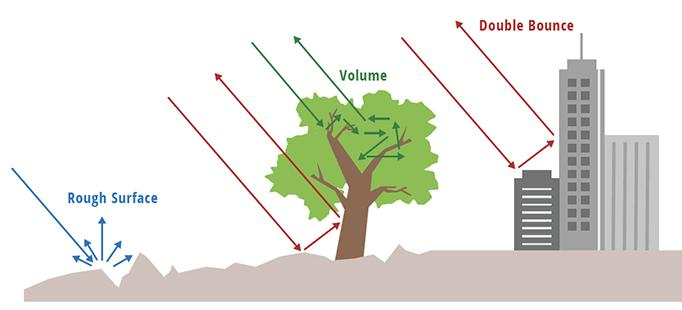
\includegraphics[width=0.8\textwidth]{utils/SARPolarization.jpg}
  \caption{Impulsi radar inviati dal satellite SAR verso la Terra e riflessi indietro.}
  \label{fig:sar_scatter}
\end{figure}  
Questo effetto di interferenza, costruttiva o distruttiva, genera un pattern granulare nell’immagine osservata, 
noto appunto come speckle. Quest'ultimo degrada la qualità visiva e radiometrica dell’immagine, rendendo più complessa l’analisi e l’interpretazione dei dati. 
Questo fenomeno è intrinseco a tutti i sistemi di imaging coerente e rappresenta un rumore di natura moltiplicativa, dipendente dal segnale, che degrada l’aspetto visivo e le prestazioni dei processi automatici di analisi dell’immagine, come classificazione o rilevamento di cambiamenti.
\section{Origine fisica dello speckle}
Il sensore SAR emette un’onda elettromagnetica e riceve il segnale retrodiffuso da una piccola area della scena, detta cella di risoluzione.  
Tale cella contiene numerosi scatterer elementari, ciascuno caratterizzato da una propria ampiezza $A_i$ e fase $\phi_i$.  
Il segnale complesso ricevuto può essere modellato come somma coerente dei contributi di tutti gli scatterer presenti nella cella \cite{6616053}:
\begin{equation}
  \makebox[\textwidth][c]{%
    $\displaystyle
      z = \sum_{i=1}^{N} A_i e^{j \phi_i}.
    $%
  }
\end{equation}
Le fasi $\phi_i$ variano casualmente a causa delle differenze di cammino ottico e, per un numero sufficientemente grande di scatterer indipendenti, il teorema del limite centrale implica che le componenti reale e immaginaria di $z$ sono variabili gaussiane a media nulla e varianza $\sigma^2 / 2$.  
In tal caso, si parla di speckle pienamente sviluppato fully developed speckle.
\section{Modello statistico}
Il modulo del segnale complesso $A = |z|$ segue una distribuzione di Rayleigh:
\begin{equation}
  \makebox[\textwidth][c]{%
    $\displaystyle
    p_A(A) = \frac{A}{\sigma^2} e^{-A^2 / (2\sigma^2)}
    $%
  }
\end{equation}
mentre l’intensità $I = A^2$ segue una distribuzione esponenziale:
\begin{equation}
  \makebox[\textwidth][c]{%
    $\displaystyle
    p_I(I) = \frac{1}{\sigma^2} e^{-I / \sigma^2}
    $%
  }
\end{equation}
Il valore medio dell’intensità è $\mathbb{E}[I] = \sigma^2$, che rappresenta la riflettività media del bersaglio o Radar Cross Section (RCS).  
Si ottiene così il cosiddetto modello moltiplicativo del rumore:
\begin{equation}
  \makebox[\textwidth][c]{%
    $\displaystyle
    I = \mu \, u
    $%
  }
\end{equation}
dove $\mu$ è la riflettività media (informazione utile) e $u$ è una variabile casuale esponenziale a media unitaria che rappresenta il rumore speckle.  
La varianza di $I$ è proporzionale al quadrato della media, quindi i pixel più luminosi sono affetti da un disturbo più forte.
Per ridurre la varianza, si può effettuare una media su $L$ osservazioni indipendenti (tecnica detta \emph{multilooking}), ottenendo una distribuzione $\mathcal{C}$ per l’intensità media $I_L$, con varianza ridotta a $\sigma^2 / L$.
\section{Effetti e problematiche}
Lo speckle riduce il rapporto segnale rumore (SNR) e ostacola l’estrazione di informazioni affidabili da immagini SAR.  
Inoltre, poiché la sua intensità è proporzionale al segnale stesso, il rumore è più evidente nelle aree ad alta riflettività.  
La sua natura coerente e moltiplicativa richiede quindi modelli e tecniche di riduzione specifiche, diverse dai filtri per rumore additivo.
\section{Tecniche di despeckling}
Negli ultimi trant'anni sono stati proposti numerosi metodi per la riduzione dello speckle nelle immagini SAR.
 I primi approcci sfruttano filti spaziali come Lee, Frost e Kuan \cite{r2024specklenoiseanalysissynthetic}.
Questi operavano direttamente nel dominio dell'immagine, cioè sui pixel, sfruttando finestre locali per stimare
 statisticamente il rumore e ridurlo. Erano strumenti semplici, poco costosi dal punto 
di vista computazionale ed efficaci ma soffrivano di un limite strutturale. Per attenuare lo speckle tendevano a 
smussare anche i dettagli fini, specialmente lungo i bordi o nelle aree eterogenee. 
Con lo sviluppo della teoria delle trasformate multisensoriale negli anni Novanta, si passò ad un approccio diverso. 
Invece di agire direttamente sul'immagine, si inziò a trasformarla in un dominio 
in cui il segnale e il rumore potessero essere seprati. Nascono così i metodi basati su trasformata, come quelli che 
usano wavelet \cite{Argenti2003}. Questi strumenti rappresentano un'evoluzione concettuale dei filtri spaziali,
perchè superano alcune loro debolezze: riescono a distinguere meglio il rumore dalle strutture significative, ad 
adattarsi a diverse scale ed a preservare in maniera più accurata bordi, texture e linee sottili. 
Tuttavia, portano con sè una maggiore complessità computazionale e la possibilità di introdurre artefatti se non 
calibrati con attenzione. Infine dato che lo speckle è un rumore moltiplicativo e non semplicemente 
additivo, se non viene trasformato prima, la wavelet può non essere del tutto efficace \cite{6616053}.
Negli ultimi anni, l’attenzione si è spostata verso metodi non locali, come il filtro Non-Local Means e l’algoritmo 
SARBM3D, adattati specificamente per il despeckling di immagini SAR. Qui l'idea è radicalmente diversa, ovvero non ci si limita più a guardare in un 
intorno locale del pixel, ma si cercano nel resto dell'immagine regioni simili e si usano queste 
corrispondenze per ridurre il rumore. In questo modo lo speckle viene attenuato in maniera molto efficace, mentre 
i dettagli strutturali si preservao quasi intatti. La qualità delle immagini risultanti è generalmente
superiore a quella ottenuta con filtri locali o multirisoluzione, ciò comporta però un costo computazionale elevato 
e la necessità di algoritmi sofisticati per gestire le similitudini tra regioni. Negli ultimi dieci 
anni si è aperta una nuova fase, spinta dall'esplosione del deep learning \cite{DL_SAR}. L'idea è che le reti neurali, in 
particolare convoluzionali o basate su autoencoder, possano imparare direttamente dai dati le caratteristiche
dello speckle e il modo migliore per ridurlo. Questo approccio non si basa più nell'assumere una distribuzione 
statistica del rumore o una struttura matematica da preservare, ma si affida alla capacità della rete di 
apprendere autonomamente dalle coppie di immagini rumorose e pulite. I risultati hanno portato ad una qualità 
visiva migliore e un eccellente preservazione dei dettagli. D'altro canto, le reti neurali hanno bisogno 
di grandi quantità di dati ben calibrati per l'addestramento e possono soffrire di scarsa generalizzazione se 
applicate a scenari diversi da quelli su cui sono state addestrate oltre che ad un costo computazionale molto elevato. 
Le performance dei modelli di despeckling non è uniforme per tutti i tipi di scenari. La loro efficacia può variare
in base alle caratteristiche statistiche del bioma come contesti di vegetazione, aree rocciose e urbane, 
poichè la distribuzione del rumore e le strutture da preservare differiscono sensibilmente. Un'immagine SAR potrebbe 
comprendere due o più tipi di biomi, ciò implica che utlizzando un unico modello di despeckling, 
indipendetemente da quale esso sia, l'immagine risultante avrà aree in cui è stata ripulita meglio e aree in cui è 
stata ripulita peggio a seconda di dove il modello per come è stato realizzato ha più facilità ad operare.
L'idea da cui nasce questa tesi è quello di unire le caratteristiche migliori di determinate tecniche di despeckling, 
in modo tale che l'immagine risultante rispecchi il più possibile la realtà di interesse. Questo tipo di approccio non va a 
reinventare la ruota, cioè non punta a realizzare un nuovo modello con cui è possibile fare despeckling, ma è mirato
a sfruttare i punti di forza di modelli già esistenti fondendo i loro risultati tramite diverse tecniche. 